% Comentarios para Plos {{{
% The manuscript LaTeX source should be contained within a single file (do not use \input, \externaldocument, or similar commands).
%
% -- FIGURES AND TABLES
%
% Please include tables/figure captions directly after the paragraph where they are first cited in the text.
%
% DO NOT INCLUDE GRAPHICS IN YOUR MANUSCRIPT
% - Figures should be uploaded separately from your manuscript file. 
% - Figures generated using LaTeX should be extracted and removed from the PDF before submission. 
% - Figures containing multiple panels/subfigures must be combined into one image file before submission.
% For figure citations, please use "Fig" instead of "Figure".
% See http://journals.plos.org/plosone/s/figures for PLOS figure guidelines.
%
% Tables should be cell-based and may not contain:
% - spacing/line breaks within cells to alter layout or alignment
% - do not nest tabular environments (no tabular environments within tabular environments)
% - no graphics or colored text (cell background color/shading OK)
% See http://journals.plos.org/plosone/s/tables for table guidelines.
%
% For tables that exceed the width of the text column, use the adjustwidth environment as illustrated in the example table in text below.
%
% % % % % % % % % % % % % % % % % % % % % % % %
%
% -- EQUATIONS, MATH SYMBOLS, SUBSCRIPTS, AND SUPERSCRIPTS
%
% IMPORTANT
% Below are a few tips to help format your equations and other special characters according to our specifications. For more tips to help reduce the possibility of formatting errors during conversion, please see our LaTeX guidelines at http://journals.plos.org/plosone/s/latex
%
% When adding superscript or subscripts outside of brackets/braces, please group using {}.  For example, change "[U(D,E,\gamma)]^2" to "{[U(D,E,\gamma)]}^2". 
%
% Do not use \cal for caligraphic font.  Instead, use \mathcal{}
% }}}

\documentclass[10pt,letterpaper]{article} % {{{
\usepackage[top=0.85in,left=2.75in,footskip=0.75in]{geometry}

\usepackage{amsmath,amssymb}
\usepackage{changepage}
\usepackage[utf8x]{inputenc}
% \usepackage{textcomp,marvosym}
\usepackage{cite}
% Use nameref to cite supporting information files (see Supporting Information section for more info)
\usepackage{nameref,hyperref}
\usepackage[right]{lineno}

% ligatures disabled
\usepackage{microtype}
\DisableLigatures[f]{encoding = *, family = * }

\newcommand{\eref}[1]{Eq.~(\ref{#1})}
\newcommand{\Eref}[1]{Eq.~(\ref{#1})}
\newcommand{\fref}[1]{Fig.~\ref{#1}}
\newcommand{\Fref}[1]{Fig.~\ref{#1}}
% color can be used to apply background shading to table cells only
\usepackage[table]{xcolor}
\usepackage{array}
\usepackage{caption}
\usepackage{multirow}
\usepackage{booktabs}
\usepackage{graphicx}
\usepackage{boldline,multirow}


\usepackage{pdfpages}
\usepackage{tcolorbox}
\usepackage{colortbl}
\usepackage[draft,inline,nomargin]{fixme} \fxsetup{theme=color}
\FXRegisterAuthor{jm}{jmm}{\color{purple}Josue}
\FXRegisterAuthor{cp}{acp}{\color{blue}CP}
\FXRegisterAuthor{cg}{cgg}{\color{red}CG}
\definecolor{C1-EN}{RGB}{0,132,170}
\definecolor{C1-FR}{RGB}{255,117,0}
\definecolor{C1-GE}{RGB}{134,0,179}
\definecolor{C1-IT}{RGB}{49,129,6}
\definecolor{C1-SP}{RGB}{162,0,0}

\newcolumntype{+}{!{\vrule width 2pt}}

% create \thickcline for thick horizontal lines of variable length
\newlength\savedwidth
\newcommand\thickcline[1]{%
	\noalign{\global\savedwidth\arrayrulewidth\global\arrayrulewidth 2pt}%
	\cline{#1}%
	\noalign{\vskip\arrayrulewidth}%
	\noalign{\global\arrayrulewidth\savedwidth}%
}

% \thickhline command for thick horizontal lines that span the table
\newcommand\thickhline{\noalign{\global\savedwidth\arrayrulewidth\global\arrayrulewidth 2pt}%
	\hline
	\noalign{\global\arrayrulewidth\savedwidth}}


% Remove comment for double spacing
%\usepackage{setspace} 
%\doublespacing

% Text layout
\raggedright
\setlength{\parindent}{0.5cm}
\textwidth 5.25in 
\textheight 8.75in

% Bold the 'Figure #' in the caption and separate it from the title/caption with a period
% Captions will be left justified
\usepackage[aboveskip=1pt,labelfont=bf,labelsep=period,justification=raggedright,singlelinecheck=off]{caption}
\renewcommand{\figurename}{Fig}

% Use the PLoS provided BiBTeX style
\bibliographystyle{plos2015}

% Remove brackets from numbering in List of References
\makeatletter
\renewcommand{\@biblabel}[1]{\quad#1.}
\makeatother



% Header and Footer with logo
\usepackage{lastpage,fancyhdr,graphicx}
\usepackage{epstopdf}
%\pagestyle{myheadings}
\pagestyle{fancy}
\fancyhf{}
%\setlength{\headheight}{27.023pt}
%\lhead{\includegraphics[width=2.0in]{PLOS-submission.eps}}
\rfoot{\thepage/\pageref{LastPage}}
\renewcommand{\headrulewidth}{0pt}
\renewcommand{\footrule}{\hrule height 2pt \vspace{2mm}}
\fancyheadoffset[L]{2.25in}
\fancyfootoffset[L]{2.25in}
\lfoot{\today}

%% Include all macros below

\newcommand{\lorem}{{\bf LOREM}}
\newcommand{\ipsum}{{\bf IPSUM}}

%\FXRegisterAuthor{cg}{cgg}{\color{red}CG}

%% END MACROS SECTION

% }}}
\begin{document}
% Autores, titulo y otros {{{
\vspace*{0.2in}

% Title must be 250 characters or less.
\begin{flushleft}
	{\Large
		\textbf\newline{Statistical analysis of 1-gram flow among Indo-European languages \cgnote{Statistical analysis of word flow among Indo-European languages}} % Please use "sentence case" for title and headings (capitalize only the first word in a title (or heading), the first word in a subtitle (or subheading), and any proper nouns).
	}
	\newline
	% Insert author names, affiliations and corresponding author email (do not include titles, positions, or degrees).
	% \\
	% \cpnote{Discutir los autores: Josue, CarlosG, FLores, CarlosP, quizá sergio? Fernanda? } 
	
	Josué Ely Molina  \ddag\textsuperscript{1,2}, %\textsuperscript{1,2\Yinyang},
	Jorge Flores      \dag \textsuperscript{2}, %\textcurrency},
	Carlos Gershenson \textsuperscript{3,4},
	Sergio Sanchez    \textsuperscript{5},
	Carlos Pineda     \ddag\textsuperscript{2,*}    % \textsuperscript{2\Yinyang},
	%Name5 Surname \textsuperscript{2\ddag},
	%Name6 Surname \textsuperscript{2\ddag},
	%Name7 Surname \textsuperscript{1,2,3*},
	
	%with the Lorem Ipsum Consortium\textsuperscript{\textpilcrow}
	
	\newcommand{\unam}{Universidad Nacional Aut\'{o}noma de
		M\'{e}xico, Mexico City, 01000, Mexico}
	% \address[1]{Instituto de F\'{\i}sica, \unam}
	% \address[2]{Centro de Ciencias de la Complejidad, \unam}
	% \address[4]{ Instituto de Investigaciones en Matem\'{a}ticas Aplicadas y Sistemas, \unam }
	% \address[6]{
	% 
	% }
	% 
	
	%\\
	\bigskip
	\textbf{1} Facultad de Ciencias, \unam \\
	\textbf{2} Instituto de F\'{\i}sica, \unam \\
	\textbf{3} Instituto de Investigaciones en Matem\'{a}ticas Aplicadas y Sistemas, \unam \\
	\textbf{4} Centro de Ciencias de la Complejidad, \unam \\
	\textbf{5} 
	Maestr\'{\i}a en Ciencias de la Complejidad, 
	Universidad Aut\'{o}noma de la Ciudad de M\'{e}xico,
	Mexico City, Mexico
	\\
	\bigskip
	
	% Insert additional author notes using the symbols described below. Insert symbol callouts after author names as necessary.
	% 
	% Remove or comment out the author notes below if they aren't used.
	%
	% Primary Equal Contribution Note
	% \Yinyang These authors contributed equally to this work.
	
	% Additional Equal Contribution Note
	% Also use this double-dagger symbol for special authorship notes, such as senior authorship.
	\ddag These authors also contributed equally to this work.
	
	% Current address notes
	% \textcurrency Current Address: Dept/Program/Center, Institution Name, City, State, Country % change symbol to "\textcurrency a" if more than one current address note
	% \textcurrency b Insert second current address 
	% \textcurrency c Insert third current address
	
	% Deceased author note
	\dag Deceased
	
	% Group/Consortium Author Note
	% \textpilcrow Membership list can be found in the Acknowledgments section.
	
	% Use the asterisk to denote corresponding authorship and provide email address in note below.
	* carlospgmat03@gmail.com
	
\end{flushleft}
% Please keep the abstract below 300 words
% }}}
\section*{Abstract} % {{{
\cpnote{Por hacer al final}
% }}}

\linenumbers
% Use "Eq" instead of "Equation" for equation citations.
% For figure citations, please use "Fig" instead of "Figure".
\section*{Introduction} % {{{

% {\color{C1-EN} {C1-EN}}
% {\color{C1-FR} {C1-FR}}
% {\color{C1-GE} {C1-GE}}
% {\color{C1-IT} {C1-IT}}
% {\color{C1-SP} {C1-SP}}
% {\color{red} \rule{\linewidth}{0.5mm}}
% \cpnote{No me gusta el inicio de la intro. Como que sugiere que hacemos el 
% estudio porque podemos. Creo qe toca pensar mejor la justificacion y abrir 
% en esa direccion. Me gusta mucho mas el segundo parrafo y quizá quisiera iniciar
% de esa manera.}
% \jmnote{Modifique el primer parrafo, el parrafo viejo quedo en el text comentado}

\cpnote{Aun no hay una justiicación de por que estudiamos lo que estudiamos. Si quieres
	lo platicamos con CarlosG la siguiente vez que nos veamos. Mientras piensa un poco y 
	si quieres platicar conmigo, lo podemos hacer.}
In recent years, the emergence and development of computational tools has
benefited various statistical studies to understand certain characteristics of
the human population. For example, we are able to predict the growth rate of a
city, the number of people who have watched a movie, the user traffic on a web
page, and even the way we use words in written language. The previous examples
are cases of the Zipf's law, formulated by George Zipf in 1940~\cite{Zipf} upon
discovering that if  the words used in a text are ranked by their frequency of
appearance, where the lower ranks belong to the most frequent words,  then the
frequency  $f$  of any word and its rank  $k$ are related by a power law of the
form $f~1/k$.




%In recent years, the field of linguistics has been benefited from the
%development of more sophisticated computational tools, helping to process a
%greater amount of data in less time and allowing the study of linguistics
%from a statistical perspective.  This statistical study began with the works
%of George Zipf~\cite{Zipf}, in them Zipf argues that if  the words used in a
%text are ranked by their frequency of appearance,  where the lower ranks
%belong to the most frequent words,  then the frequency  f  of any word and its
%rank  k are related by a power law of the form f~1/k. The previous expression
%is known as  Zipf’s law, and it has not only been tested on language datasets,
%Morales et al.~\cite{Morales_epj} have also proved on sports and games data,
%and Cristelli et al.~\cite{Cristelli_zipfgdp} on the gross domestic product of
%several countries,  wealth of American citizens,  and population of cities.

Zipf's law has been mostly used to study the structures of language,
nonetheless, not enough studies have been done to understand the historical and
cultural features that language provides. One way to begin such a study is by
noting that the languages themselves are mixed, since within the vocabulary of
a language, from other languages are continuously added.

% %Although Zip’s law has opened several statistical studies in linguistics, nowadays few studies have been done about how within the vocabulary of a language, words from the language itself and from other languages are mixed
% \cpnote{Creo que podemos aca hablar mas de un mixing de cultura. Irnos de cosas generales a cosas particulares. Ahora, gracias a google ngram podemos aproximarnos a este problema mediante el lengauje}.
% \jmnote{modifique un poco este parrafo,  considero que el mixing del lneguaje y la cultura esta tratado en los sig parrafos}

Currently in the Spanish language, there are words from English 
that do not have a translation or that sometimes displace those that already
exist in Spanish.  For example, for native Spanish speakers it is common to
hear the word \textit{marketing} instead of its translation \textit{mercadeo}
when dealing with economic or business issues; also the word \textit{online}
has replaced \textit{en línea}, when referring to issues related to the
internet, a word officially adopted in Spanish.

This trending has not only affected Spanish,  but also other languages that are
being influenced by topics where English is the main and common language for
communication. However, in different periods of time, the flow of words came
from other languages. D’Amore~\cite{Damore_influencia_mutua} discusses with linguistic rigor the
flow of words between English and Spanish,  showing historical  and cultural
causes that allowed such flow; in addition to mentioning the influence of
Arabic in Spanish and French in English. \cpnote{Hay mas referencias, o es un 
	caso singular?}

In this work, we use the Google Books N-gram~\cite{ngramv} dataset of the most
frequent words in books published in  English, French, German, Italian and
Spanish languages.  With that dataset,  we develop an algorithm that identifies
the words of one language  and that are being used exactly with the same 
spelling by others. Once these words
have been classified, we construct two models to quantify  the influence that
one language has had on another during the 20th century. The first model, we
count the number of new words that a language received from another, while in
the second method, we develop the concept of the use of one language in
another,  from quantifying the relative frequency of  the words of a language
that are being used in another language. In both we identify historical, social
and cultural causes that are responsible for the flow of words.

Next, we use the concept of rank diversity,  that shows the number of words
occupying a certain rank across the time. This study shows that  regardless of
who is the language the flow comes from or who language receives them,  the
lower ranks are always occupied by fewer  words, and as the rank increases the
diversity curve also increases as a logarithmic. 

\cpnote{Obvio aca toca poner algunos caveats y discutir la seccion de la estabilidad}

\cgnote{Uno de los caveats es que como hacemos comparaciones automatizadas de cadenas (llam\'emosle ``blind big data''), nuestras comparaciones son puramente de palabras completas, ya no digamos sem\'anticas. Por ejemplo, estamos limitados para estudiar influencia de y hacia ruso, simplemente porque tiene otro alfabeto. Hay otras transformaciones que no detectamos, e.g. en espa\~nol se agrega `e' antes de `sp' (especial/special). Y tambi\'en hay casos donde la influencia puede ser de otros idiomas, e.g. Lat\'in, aunque en otros casos se puede detectar por d\'onde lleg\'o la influencia (e.g. sushi?). Otra limitante es que nos enfocamos en palabras de uso frecuente. S\'olo decir que los estudios comparativos de ``insightful small data'', donde humanos identifican manualmente flujos de palabras seguir\'an siendo \'utiles y necesarios. }

%\begin{eqnarray}
%\label{eq:schemeP}
%	\mathrm{P_Y} = \underbrace{H(Y_n) - H(Y_n|\mathbf{V}^{Y}_{n})}_{S_Y} + \underbrace{H(Y_n|\mathbf{V}^{Y}_{n})- H(Y_n|\mathbf{V}^{X,Y}_{n})}_{T_{X\rightarrow Y}},
%\end{eqnarray}
% }}}
\section*{Metodology} % {{{

For the development of this work,  we used the Google Books Ngram data set~\cite{ngramv}.
This dataset contains the usage frequency, for each year and language, of
the most used ``$n$-grams'' in the books of Google Books. 
``$n$-grams'' are the words or set of words that make up the text of a
book, where the number $n$ indicates the number of words that make up the gram,
being a 1-gram an individual word, a 2-gram a phrase composed of two 1-gram,
3-gram the set of three 1-gram and so on.
We removed certain words that did not contributed to the analysis. 
We eliminated articles, pronouns, propositions and conjunctions (all 
of which are functional words), since these
serve to give a structure to the message;  then we consider content words as
nouns, adjectives and adverbs, which are responsible for the information in the
message. Although the names of people, countries and cities are also considered
functional words, we did not eliminate them, since for some languages these
words show a cultural trend that we have decided to take into account. \cpnote{Preguntar
a josue donde vio qeu los proper nouns son functional words}
From this data set, and after cleaning the data, the lists of the five thousand
most used 1-grams each year
between 1740 and 2009 were extracted for the English, French, German, Italian
and Spanish languages.
We are performing this cut as all the lists of the six languages (between 1740
and 2009), have at least this amount of 1-grams.
In each list, the words are ranked according to their
frequency of appearance, where the most frequent words have the lowest ranks.

% \cpnote{Creo qe se tienen que unir los parrafos y decir de done salen esaos
% 	ngrams, que son de libros escaneados}
% 

To determine the presence of one language in another, an algorithm was
developed to find the words that are common between at least two languages,
these must have exactly the same spelling. These words were defined
as \textit{migrant words}. 
A migrant word is associated with a \textit{source language} and a
\textit{receiving language}, where the source language is the one where the
word appeared for the first time within the most used words,
while the receiving language is the one where the word is also present, being a
different set from the source language. 
To determine the source language, we established that this will be the language
where the word appeared for the first time within the five thousand most used
words; in the case of a migrant word has appeared in the same year in two or
more languages, the source is the one where the word has the lowest rank.


The previous criteria of looking for words with the same writing and later
associating them with a source language, is not perfect there are some cases
that our method did not detect and were established as mistakes. One of the
most common errors was finding words with the same writing, but with different
meanings. For example,  \textit{mayor} in English refers to the representative
of the government in a locality, while in Spanish, mayor is an
adjective to indicate that something is bigger or older.  Another recurring
error was to not distinguish words with the same meaning but with different
endings. For example, the word \textit{imagine} is written \textit{imaginer} in
French and \textit{imaginar} in Spanish.  Finally, in some cases, the authentic
source language is some other language for which there is no information in the
data set, for example the word  natural comes from Greek, but there is no data
from Greek language in the google books $n$-grams data set, consequently this
word was associated with English as its source language.

The above errors were detected by individually analyzing each of the migrant
words and their corresponding source and receiving languages. One way to have
cleaner data is by consulting an expert in each language, who review the words
and decide which ones were classified properly, however, this is not practical
since if there were more languages in the database, it would be necessary to
consult an expert for each language. Notwithstanding of this requirement to
regulate errors, we established a method to determine the importance (weight)
of these errors in the results, that will show in the following sections. 
% }}}
\section*{New words} % {{{
% Results and Discussion can be combined.
 
The purpose of this work is to establish the influence that one language has on
another. A first method to quantify such influence is by counting the
\textit{new migrant words} (NMW). These are words that appear for the first time in a
receiving language and that come from an unique  source language.


We study the flow of NMW, per decade, in two ways. First, we
count the number of NMW that a fixed language exports as a source
language. Second, counting, for a fixed language, the number
of new migrant words. In this second way, we can study from 
which language are the NMW coming. The results are presented in 
\Fref{fig.NMW_A} for each decade of the 20th century. 

% We count new migrant words in two ways. First, by counting the number
% of new words for a fixed receiving language in a given decade. 
% receiving language, then for each decade, how many new migrant words from the
% other source languages have appeared are counted. The second way is to take one
% language as the source language for the new migrant words, and count how many
% of them have appeared in the other receiving languages.
% 
% Counting new migrant words is done in two ways. First, taking a language as the
% receiving language, then for each decade, how many new migrant words from the
% other source languages have appeared are counted. The second way is to take one
% language as the source language for the new migrant words, and count how many
% of them have appeared in the other receiving languages.

From this figure, we can see that the English language has
migrated on average three times more words than it has received, where the
greatest influence of English occurred between the 1940s, 1990s and 2000s.
Consequently, the
largest proportion of migrant words in the other languages come
from English. French, German, Italian and Spanish have received more words
during the second half of the century, after the end of World War II.
\cpnote{CarlosG, el analisis que se hace de esta figura aun esta muy precario. 
Creo que podemos ver la figura, y platicar tantito a ver que mas podemos decir de ella.}¸

\begin{figure} % {{{
\begin{adjustwidth}{-1.2in}{0in}
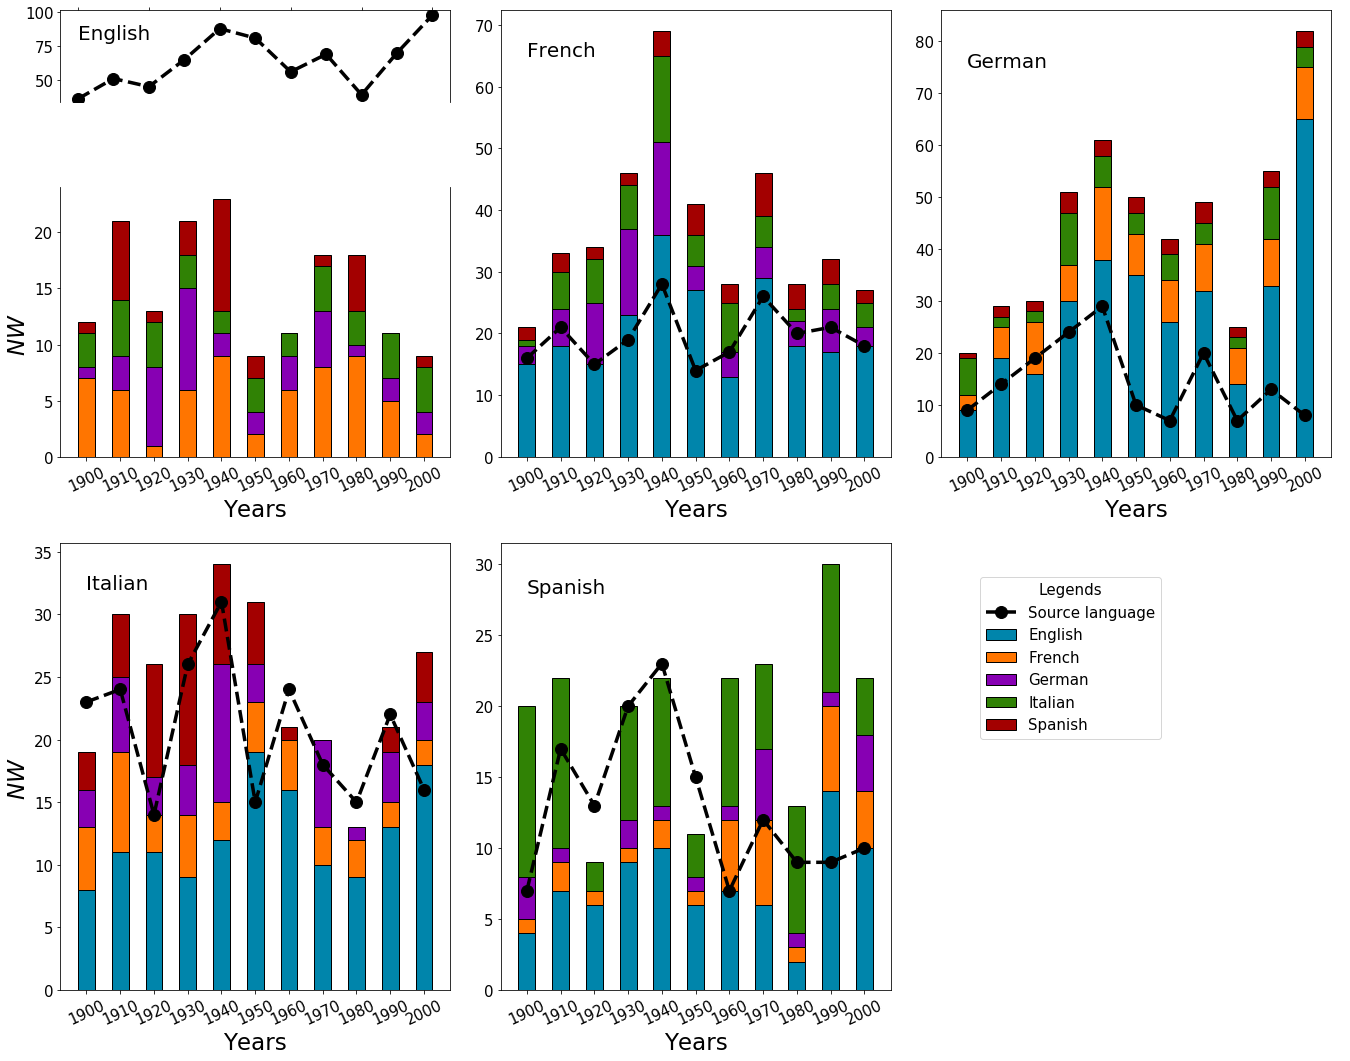
\includegraphics[scale=.35]{NW_A.png}
% \caption{{\bf New migrant words that migrate from one source language to the
% different receiving languages.} Among language such as sources (dotted plot)
% and receivers (bar plot) of new words, only English language has been the
% language that has migrated more words than it has received. Consequently, the
% largest proportion of migrant words in the other languages come
% from English. French, German, Italian and Spanish have received more words
% during the second half of the century, after the end of World War II.	
% \cpnote{Explicar la curva punteada, poner los colores aparete, digamos en una
% leyenda como un sexto grafico un poco, y describir mejor y analizar tantito
% (una frase).}
% \jmnote{listo}
% }
\caption{{\bf New migrant words, per language and per decade.} 
NMW are consider for each language. Each panel contains one language. 
The dotted line displays the number of NMW that originate in the 
corresponding language, and the bars the NMW coming to that language, 
separated by the origin of the different NMW. 
% 
% Among language
% such as sources (dotted plot)
% and receivers (bar plot) of new words, only English language has been the
% language that has migrated more words than it has received. 	
% \cpnote{Explicar la curva punteada, poner los colores aparete, digamos en una
% leyenda como un sexto grafico un poco, y describir mejor y analizar tantito
% (una frase).}
% \jmnote{listo}
}
% 
\label{fig.NMW_A}
\end{adjustwidth}
\end{figure} % }}}
	
Analyzing the lists  of 
% After counting, we analyzed each of the 
migrant words, we realized that
these can be grouped into semantic fields. According to~\cite{semantic_oxford},
a semantic field is a set of words that are related based on their meaning.
% then we can group the new migrant words by their meaning.
Table~\ref{tab.new_words} shows the words grouped by semantic fields, as well as
the pairs of source language and receiving language involved. We note that the
year of appearance (or in the years around) of the migrant words, a historical
or cultural event occurred that is related to the semantic field. For example,
between 1930 and 1940, words historically related to the Second World War
migrated between all languages; while since the 1990s the words migrant refer
to the fields of technology and globalization.  
% \jmnote{agregar mas sobre la tabla??}¸

\begin{table}[htb] % {{{
\centering
\resizebox{\textwidth}{!}{
\begin{tabular}{@{}cV{4.5}cV{4.5}cV{4.5}c@{}}
\textbf{Semantic Field} & \textbf{New migrant words}
      & \textbf{Source language} & \textbf{Receving laguage} \\
\hlineB{4.5}
\multirow{2}{*}{World War I} 
   & \begin{tabular}[c]{@{}c@{}} \\ allemagne,  austro,\\  russie, versailles.\end{tabular} 
   & FR    & \begin{tabular}[c]{@{}c@{}}\\IT (1910, 1920), GE (1920).\end{tabular} \\
 & kaiser, reich. & GE   & FR (1910). \\
\hlineB{4.5}
	\multirow{5}{*}{World War II}                                                                    & \begin{tabular}[c]{@{}c@{}}catastrophe, churchill,\\ nazis, stalin, territories.\end{tabular}                                                           & EN                       & \begin{tabular}[c]{@{}c@{}}FR (1940), \\ IT (1940).\end{tabular}                                                     \\
	& \begin{tabular}[c]{@{}c@{}}berchtold, bestimmungen,\\  hitler, kaiser, lenin, \\ minister, regierung.\end{tabular}                                      & GE                       & \begin{tabular}[c]{@{}c@{}}EN (1930), FR (1940),\\ IT (1930, 1940),\\ SP (1930).\end{tabular}                        \\
	& \begin{tabular}[c]{@{}c@{}}duce, mussolini, \\ panzer, regime.\end{tabular}                                                                             & IT                       & \begin{tabular}[c]{@{}c@{}}EN (1930), FR (1930),\\ GE (1930, 1940),\\ SP (1930).\end{tabular}                        \\
	
	\hlineB{4.5}
	Aftermath of WWII                                                                                & onu, urss, vietnam                                                                                                                                      & FR                       & SP (1960, 1990).                                                                                                     \\
	\hlineB{4.5}
	\multirow{2}{*}{\begin{tabular}[c]{@{}c@{}}Important surnames \\ in academic areas\end{tabular}} & poincare.                                                                                                                                               & FR                       & IT (1920).                                                                                                           \\
	& \begin{tabular}[c]{@{}c@{}}bach, beethoven, engels, \\ freud, hegel, heidegger, \\ marx, mozart, nietzsche.\end{tabular}                                & GE                       & \begin{tabular}[c]{@{}c@{}}EN (1930), FR (1900-1980),\\ IT (1900, 1940, 1970),\\ SP (1930, 1970, 1980).\end{tabular} \\
	\hlineB{4.5}
	\multirow{2}{*}{\begin{tabular}[c]{@{}c@{}}Ideologies and \\ political terms\end{tabular}}       & \begin{tabular}[c]{@{}c@{}}burgueoise, diplomatie, \\ empire, politique.\end{tabular}                                                                   & FR                       & GE (1910-1930).                                                                                                      \\
	& \begin{tabular}[c]{@{}c@{}}capitalista, comunista, fascismo, \\ marxismo, socialista, terrosismo.\end{tabular}                                          & IT                       & SP (1910, 1930, 1960, 1980).                                                                                         \\
	
	
	\hlineB{4.5}
	Economy                                                                                          & \begin{tabular}[c]{@{}c@{}}depression, dollar, economic, \\ economy, financial, investment, \\ market, marketing, value.\end{tabular}                   & \multirow{4}{*}{EN}      & \begin{tabular}[c]{@{}c@{}}FR (1950), \\ GE (1930, 1990, 2000),\\ SP (1980-2000).\end{tabular}                       \\
	Technology                                                                                       & \begin{tabular}[c]{@{}c@{}}digital, internet, mail, \\ online, software.\end{tabular}                                                                   &                          & \begin{tabular}[c]{@{}c@{}}FR (1990), GE (1990),\\ IT (1990, 2000), \\ SP (1990, 2000).\end{tabular}                 \\
	Globalization                                                                                    & \begin{tabular}[c]{@{}c@{}}business, customer, management, \\ market, marketing, standars.\end{tabular}                                                 &                          & \begin{tabular}[c]{@{}c@{}}FR (2000), GE (1990, 2000),\\ IT (2000),  SP ( 2000).\end{tabular}                        \\
	\begin{tabular}[c]{@{}c@{}}Presidents of the\\ United States of\\ America\end{tabular}           & \begin{tabular}[c]{@{}c@{}}roosevelt, truman, kennedy,\\ johnson, nixon, reagan,\\ bush, clinton.\end{tabular}                                          &                          & \begin{tabular}[c]{@{}c@{}}FR (1960, 1970), GE (1930,1940),\\ IT (1940),  SP (1940-1990).\end{tabular}               \\
	\hlineB{4.5}
	Medicine                                                                                         & \begin{tabular}[c]{@{}c@{}}anemia, anestesia, colesterina,\\ endovenosa, gastrica, lepra\\ metabolismo, sintomatologia, virus,\\ vitamina.\end{tabular} & \multirow{2}{*}{SP}      & \begin{tabular}[c]{@{}c@{}}EN (1940), GE (1990,1940),\\ IT (1920, 1930),\end{tabular}                                \\
	\begin{tabular}[c]{@{}c@{}}Latinoamerican countries \\ and cities\end{tabular}                   & 
	\begin{tabular}[c]{@{}c@{}}argentina, aires, buenos,\\ chile, panama.\end{tabular}                                                                      &                          & \begin{tabular}[c]{@{}c@{}}EN (1910, 1940), FR (1910), \\ IT(1900).\end{tabular}                                    
\end{tabular}%
}
\caption{\textbf{New migrant words.} 
\cpnote{Agregar descripcion mas detallada}
We use the following abbreviations: EN for English, FR for French, GE for German, IT for
Italian and SP for Spanish. 
}
\label{tab.new_words}
\end{table} % }}}

These kind of groupings allow us to say in which areas the languages are most
influential and the reason for the migration of words. The English language has
migrated words to others thanks to the development of technology and
globalization in the last thirty years, the French, Italian and German
languages after the war events of the 20th century, in addition to the academic
influence of German by the surnames of German-speakers who excelled in academic
areas; finally Spanish after economic crises in Latin American
countries~\cite{crisis_chile}. \cpnote{CarlosG, de nuevo, tu eres bueno para describir
estas cosas. Sería un buen punto para agregar.}

% }}}
\section*{Accumulated words} % {{{
% Intro y definicion {{{

The previous results show that words travel from one language to another in
groups belonging to a common semantic field. Nevertheless, we still cannot
associate them with a number that quantifies how much influence has one
language on another.

To obtain such a number, we will focus on migrant words in the years after the
first year they migrated, observing how their frequency varies over time. For
example, a migrant word will begin to be influential if its frequency increases
over time. Since we are dealing with groups of words, we define as accumulated
migrant words, those words with source language $A$ that already appeared in a
receiving language $B$, and for a given year they do so again.

Let us define $J_{AB}$ as the rankings of the set of words in $B$ that migrated
from $A$ and define also the frequency $f(j)$ of a word with ranking $j$. We now
add the frequencies of the accumulated
migrant words of $A$ to $B$ at a year $t$ and normalize the this quantity by
dividing it by the frequency of the five thousand words that make up the list.
\begin{equation}
\label{ec.fuso}
\underset{ \text{\tiny A} \to  \text{\tiny B} }{U}(t) = \frac{\sum_{j}
f(j)}{\sum_{k=1}^{5000} f(k)}.
\end{equation}


% take the list of the most used words of $B$ in a year $t$, we add the
% frequencies of the accumulated
% migrant words of $A$ that have a rank $j$; we normalize the this quantity by
% dividing it by the frequency of the five thousand words that make up the list.
% \begin{equation}
% \label{ec.fuso}
% \underset{ \text{\tiny A} \to  \text{\tiny B} }{U}(t) = \frac{\sum_{j} f(j)}{\sum_{k=1}^{5000} f(k)}.
% \end{equation}

% If we take the list of the most used words of $B$ in a year $t$ (the words are
% ranked according to their frequency), we add the frequencies of the accumulated
% migrant words of $A$ that have a rank $j$; we normalize the this quantity by
% dividing it by the frequency of the five thousand words that make up the list.
% \begin{equation}
% \label{ec.fuso}
% \underset{ \text{\tiny A} \to  \text{\tiny B} }{U}(t) = \frac{\sum_{j} f(j)}{\sum_{k=1}^{5000} f(k)}.
% \end{equation}
% 
We define this new value as the \textit{use} of $A$ in $B$, and interpret is value
as a measure of influence. It will then be said that the influence of $A$ has increased on
$B$, if in an interval of time $\Delta t$ the use of $A$ on $B$ increases.
Finally, to quantify the change in use within a time interval, the term ratio
of words per year (wpy) will be used, obtained by dividing $\Delta U$  by
$\Delta t$.

We obtained the accumulated migrant words for all possible combinations of
source and receiving languages from 1740 to 2009.  Afterwards, we calculated
the use, \eref{ec.fuso},  for each pair of languages between 1900 and 2009, so
as to have a time period (1740-1899) to build a large enough dataset to have
meaningful migrant words. The results are presented in \fref{fig.UT_art}, 
grouped by source language. 


% 
% Then in each combination we applied
% the equation~\ref{ec.fuso} to realize the use in the years between 1900 and
% 2009. 
\cpnote{Preguntar a Josue donde va esto y poner en el lugar apropiado}
In addition, to name some combination of source
and receiving languages, two abbreviations will be used, the first being the
source language of the accumulated migrant words, and the second the receiving
language of them, for example EN-GE, means the migrant words from English that
are present in the German.


% To simplify the notation in the plots we establish a set of abbreviations to
% distinguish the languages: EN for English, FR for French, GE for German, IT for
% the Italian and SP for Spanish. In addition, to name some combination of source
% and receiving languages, two abbreviations will be used, the first being the
% source language of the accumulated migrant words, and the second the receiving
% language of them, for example EN-GE, means the migrant words from English that
% are present in the German.

% We obtained with the previous method, the accumulated migrant words among all
% the possible combinations from a source language to a receiving language, in
% the 269 years (1740-2009) of the dataset. Then in each combination we applied
% the equation~\ref{ec.fuso} to realize the use in the years between 1900 and
% 2009. To simplify the reading we establish s set of abbreviations to
% distinguish the languages, EN for English, FR for French, GE for German, IT for
% the Italian and SP for Spanish. In addition, to name some combination of source
% and receiving languages, two abbreviations will be used, the first being the
% source language of the accumulated migrant words, and the second the receiving
% language of them, for example EN-GE, means the migrant words from English that
% are present in the German.

% The migrant accumulated words between pairs of language were ordered by the
% year in which they appeared and in descending order in their frequency.
% Therefore the first place in the ranking is occupied by the most frequent word
% in that year, the second for the second most frequent, and so on.

% \cpnote{Aca voy}
% Fig~\ref{fig.UT_art} shows the use of a source language, in all receiving
% languages, as the use in each case may have a different scale, the data were
% normalized by dividing them by their average value, this with the intention of
% observing in which time interval the use was more affected (increase or
% decrease more than in the others), since this will indicate that accumulated
% words were more or less influential. 


\begin{figure}[!h]
	\begin{adjustwidth}{-2cm}{1cm}
		\centering
		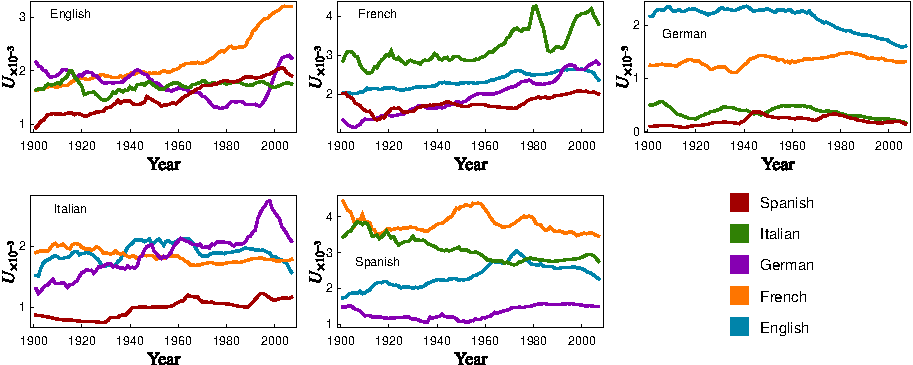
\includegraphics{images/usoFinal.pdf}
% 		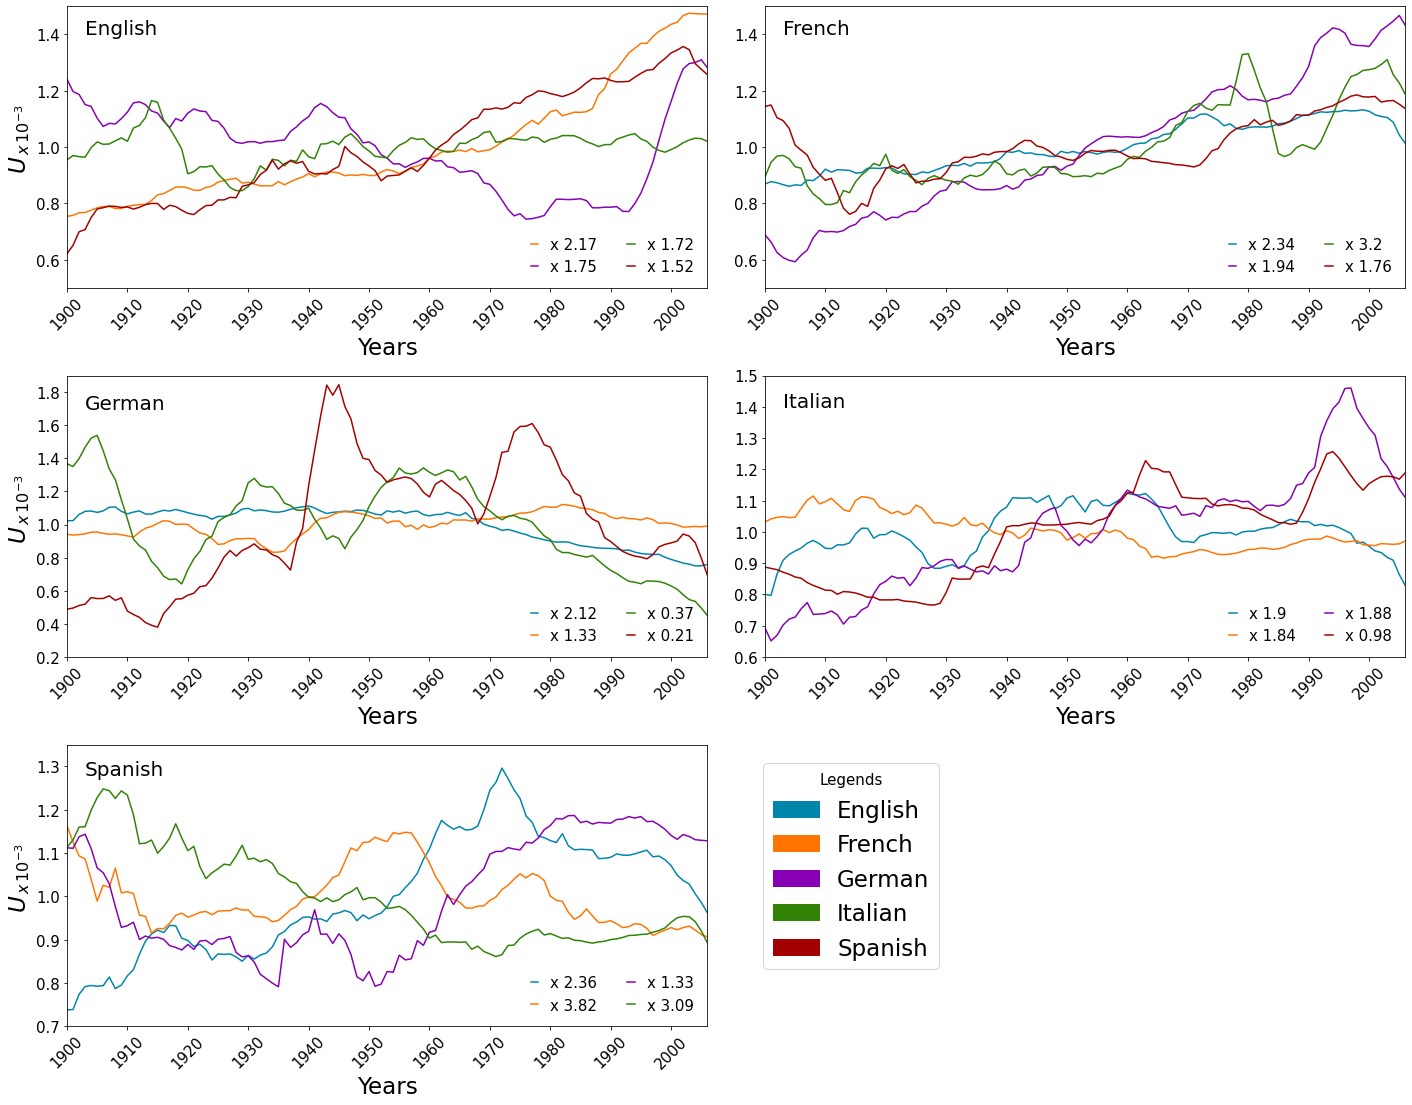
\includegraphics[scale=0.38]{USO_A.png}
		\caption{{\bf The Use among languages.} \cpnote{HAcer el caption
cuando termine el articulo} All language pairs..... Decir que una descripcion para 
cada curva se da en el texto principal}
		\label{fig.UT_art}
	\end{adjustwidth}
\end{figure}
% }}}
\subsubsection*{English} % {{{

The use of English in French and Spanish has increase steadily in the last century
whereas in Italian, it has maintained a constant level. 
An increase in the use  in German was until 1990. We associate the cause of these increases
with the emergence of the United States as a world power, after finishing the
World War II (WWII) and  impose its economic model as well as the development
of science and
technology. The accumulated migrant words that are present in all receiving
languages are \textit{capital}, \textit{dollar}, \textit{invesment},
\textit{relations}, \textit{market}, \textit{company}, \textit{development},
\textit{financial},  \textit{institutions}, \textit{internet}, \textit{windows}
and \textit{software}. Those can again be associated with semantic fields such
as economics, technology, and globalization.

% }}}
\subsubsection*{French} % {{{

The increase in the influence of French in the other languages occurred in
English between 1920 and 1970, in German between 1900 and 2009, and in Spanish
between 1970 and 1995. In these years the words that increased its frequency
are from the semantic fields of religion such as \textit{dieu} ,
\textit{évêque}, \textit{dime}, \textit{religion}, \textit{saint} and
\textit{église} (iglesia); while \textit{reine}, \textit{forteresse},
\textit{napoleon}, \textit{guerre}, \textit{imperiale}, \textit{bastille},
\textit{royal} and \textit{bourgeois} are from French Revolution.

In Italian between 1950 and 1970, in addition to the above
words,\textit{raisins}, \textit{vin}, \textit{vignoble} y \textit{recolte} were
found, the common meaning of which is the wine industry, a common industry in
France and Italy.

% }}}
\subsubsection*{German} % {{{

Spanish and French,  between 1930 and 1945 were the languages where German had the greatest
increase among all receiving languages; 
in both, the words that are present are the surnames of German-speaking
characters who excelled in academic areas, such as \textit{Marx},
\textit{Freud}, \textit{Heidegger}, \textit{Nietzsche}, \textit{Hegel},
\textit{Engels} and \textit{Mozart}.

In English and Italian, the biggest change was between 1960 and 2009, where the
use of German decreased. In this period the words that lost influence
\cpnote{Josue, a que te refieres con palabras que han perdido influencia?} are
referred to the World War II, among them \textit{Berlin}, \textit{Marx},
\textit{Hitler}, \textit{Lenin}, \textit{testen}  and \textit{reich}.
% }}}
\subsubsection*{Italian} % {{{


The influence of Italian came mainly from two semantic fields, the WWII with
\textit{Mussolini}, \textit{fascismo}, \textit{battaglia}, \textit{regime},
\textit{sociale} and \textit{liberale}; and the religion with \textit{santo},
\textit{suora} and \textit{cattedrale}. These semantic fields are
responsible for the increase in English between 1930 and 1940, in German
between 1950 and 1995, and in Spanish between 1930 and 1960.
\cpnote{Josue, hay un pico fuere en la influencia del italiano en el aleman como 
en 1990. Te queda facil ver que es?}

In French, Italian has the lowest influence, where the aforementioned words
began to be less frequent between 1940 and 1960.
% }}}
\subsubsection*{Spanish} % {{{

The influence of Spanish in English between 1920 and 1970, was due to
historical and cultural facts. Names of Latin American  countries such as
\textit{Mexico}, \textit{Panama}, \textit{Chile}, \textit{Cuba}, \textit{Peru},
\textit{Colombia}, \textit{Argentina} and its capital \textit{Buenos}
\textit{Aires};  and states in the United States  where a large part of the
Spanish-speaking population is concentrated as \textit{California} and
\textit{florida}, are an important part of words that appeared in 
other languages. 

In German after WWII, and in French between 1930 and 1955, the mainly words
involved in that increse are, \textit{terapia}, \textit{anemia},
\textit{lepra}, \textit{tumor}, \textit{syphilis}, \textit{virus} and
\textit{renal}. \cpnote{CarlosG, Josue, Hay alguna explicacion a este fenomeno?}

% }}}
% }}}
\section*{Rank diversity} % {{{

In the previous sections, we quantified the influence of a language on another. However, 
one can wonder about how the migrant words change in time. Are the most important words
the same, or do they change? In fact, 
since the accumulated migrant words are organized by year, and at the same time
in each year the words are ordered in ascending order in rank, then over time,
the same rank can be occupied by different words. One way to quantify
this change is through rank diversity $d(k)$~\cite{iplosone}. This quantity is
defined as the number 
of different elements that occupy rank  $k$ within the same data set, divided
by the number of time slots considered.
%  how many
% different elements can occupy the same rank within the same corpus is through
% rank diversity $d(k)$ \cpnote{this last sentence belongs to a paragraph introducing rank
% 	diversity. I think that we must start saying the idea that we want to quantify. That, 
% 	in a paragraph. Then another paragraph that really introduces the measure, which I think
% 	is still laking. Maybe a single paragraph that contains both ideas.}.
% \cpnote{
% Decir que aca mencionamos antes como varia el volumn de la la influencia, pero
% aca nos preguntamos como varian las palabras en si.  Why are we
% interested in rank diversity that has not been understood in the previous
% sections?}
% Since the accumulated migrant words are organized by year, and at the same time
% in each year the words are ordered in ascending order in rank, then over time,
% the same rank can be occupied by different words. One way to quantify how many
% different elements can occupy the same rank within the same corpus is through
% rank diversity $d(k)$ \cpnote{this last sentence belongs to a paragraph introducing rank
% 	diversity. I think that we must start saying the idea that we want to quantify. That, 
% 	in a paragraph. Then another paragraph that really introduces the measure, which I think
% 	is still laking. Maybe a single paragraph that contains both ideas.}.
Rank diversity has been used in datasets of the most used words in six
Indo-European languages~\cite{iplosone}, in sports and game classifications \cite{Morales_epj}, 
and in many other datasets~\cite{Iniguez2022}. 
Although in
each case the criteria for establishing a ranking are different, in both there
is a common result: for the same set of data that have had different rankings
over time, it is true that the lowest ranks are always occupied by fewer
elements, thereby as the range increases, the number of elements that occupy it
also does them.

\begin{figure} % {{{
% \begin{adjustwidth}{-2.5cm}{1cm}
\centering
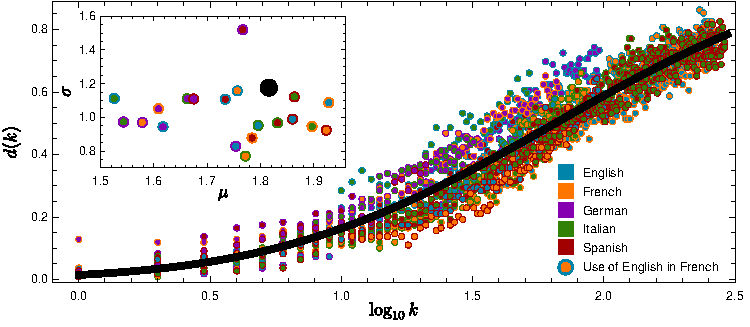
\includegraphics[scale=1]{images/Diversity.pdf}
% 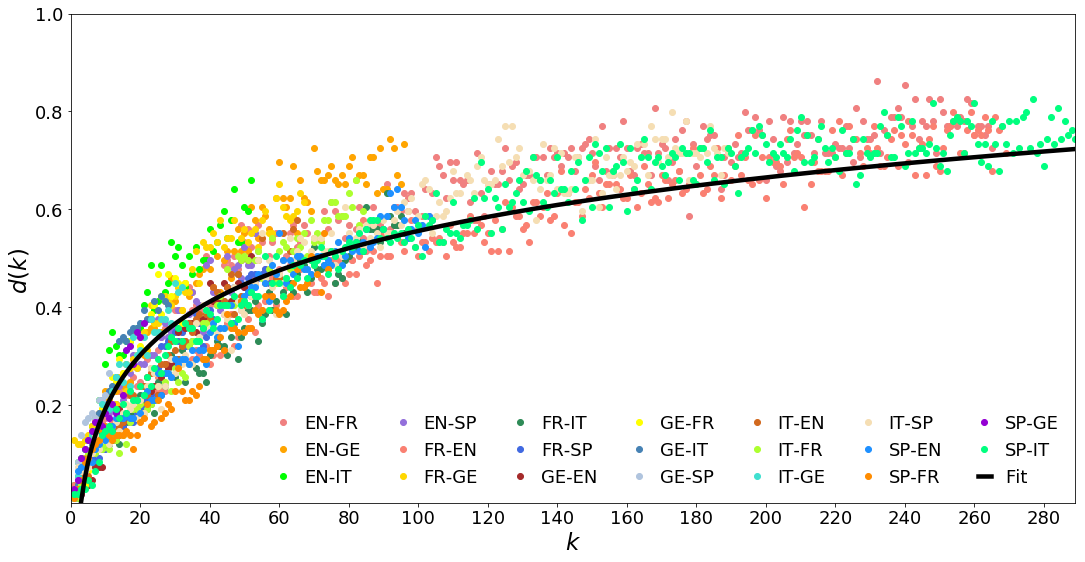
\includegraphics[scale=.38]{DR_art.png}
\caption{{\bf Rank diversity of accumulated migrant words among languages.} 
Diversity for all pairs of languages. Each pair is well fitted by the 
sigmoid proposed in \eref{eq:sigmoid}, with fitting parameters $\mu$ and $\sigma$
reported in the inset. As a reference, we show a global sigmoid (in black)
obtain by fitting all data points. Its fiting parameters are also shown in the
inset as a black dot. 
% 
% All
% language pairs conform the sigmoid curve proposed in 
% 
% 
%  show a logarithmic behavior regardless of the number of ranks
% where the rank diversity was applied. The reliability of the fit to a
% logarithmic curve of the 20 combinations is on average $R^{2}= 0.88 \pm 0.04$.
% \cpnote{Cambiar la figura cuando me ponga de acuerdo con josue quizá si ponemos
% tabla aca}
}
\label{fig.DR_art}
% \end{adjustwidth}
\end{figure} % }}}
After calculating the rank diversity for each source and receiving
language pair, the diversity values resemble a sigmoid curve, as can be
seen in Fig~\ref{fig.DR_art}. The proposed the curve is the
cumulative of a Gaussian centered at $\mu$ and with 
deviation $\sigma$, i.e.  
\begin{equation}
\Phi_{\mu,\sigma}(\log_{10} k)=\frac{1}{\sigma\sqrt{2\pi}}
   \int_{-\infty}^{\log_{10}k}\exp\left(-\frac{(y-\mu)^2}{2\sigma^2}\right) {\rm d} y,
   \label{eq:sigmoid}
\end{equation}
The parameters $\mu$ and $\sigma$
are obtained with a linear regression. 
% If $ a_{k} $ represents the
% value of the adjustment equation when evaluating it in the range $ k $, $ d_
% {k} $ is the diversity obtained for the same range and $\bar{d} $ is the
% average of all values of the diversity, then
% $R^{2}=1-\sum_{k=1}(d_k-a_k)^{2}/(d_k-\bar{d})^2$.	
% \cpnote{Creo qeu acá falta información. Si se calcularon, quizá se puede reportar. 
% O si no, para que lo decimos? Lo miso con las $R^2$, quizá ver si una tabla vale la pnena 
% poner. Discutir con Josue}
% Fig~\ref{fig.DR_art} also shows the plot of $d(k) = 0.16\ln(k) -
% 0.17$, obtained after averaging the coefficients $\alpha$ and $\beta$
% corresponding to each language pair. 
It is observed that the behavior of
diversity increases as the rank also increases, regardless of whether the
corpus has few or many ranks ($14$ in German-Spanish, $290$ in Spanish-Italian,
etc). With this, it can be concluded that, the migrant accumulated words in the
middle and high ranks are the ones that tend to change their position the most
within a ranking over time.

% An final observation is that 
% The method of the use of one language in another, showed that
% the words of certain semantic fields decrease their rank if the use tends to
% increase.
% \cpnote{Entender de donde se saca esta conclusion}
% Nevertheless, the inverse case cannot be concluded, that is, we do not know if
% the use of a language increases as a consequence of a group of words decreasing
% its rank, nor do we know how stable is the use among languages if certain words
% were not taken; since within the accumulated words of one language in another,
% only a few belong to a specific semantic field.


% }}}
\section*{Robustness} % {{{
The method we used to build the set of migrant words relied on words having {\it
exactly} the same spelling when going from one language to another. We know 
that that is not always the case. Some words change their spelling. For example
the word {\it parquear} in Spanish comes from to the verb {\it to park} in
English. 


To check the stability of the results presented and the importance of
omitting certain words, we proceeded as follows. 
Take the original set (the one obtained in the previous section) of the
accumulated words of a pair of source language and
receiving language, and from this set, eliminate a certain group of words, in order
to obtain a reduced set; in both,  equation~\ref{ec.fuso} is used to obtain the
modified
use between the years 1900 and 2009.
The next thing is to determine how similar the use of both sets are. We
normalized the values of both sets, after dividing them by the average value of
each one; then for each year $t$ we obtain the distance between each value of
original use $u_{t}$ and its corresponding value in reduced use $r_{t}$. The
average of them gets the \textit{average distance} $\left\langle D
\right\rangle$, which will be the one that quantifies the similarity of the
results, indicating a greater similarity if it is close to zero. This 
distance is defined as 
\begin{equation}
\left\langle D \right\rangle  = \frac{1}{N}\sum_{t=1}^{N} \left| u_{t} - \tilde u_{t} \right|  
\label{ec.Davg}
\end{equation}
where $u(t)$ is the original normalized usage and $\tilde u(t)$ is the reduced,
normalized usage.

\subsection*{Elimination characteristics}

To answer how stable the sets are if we altering them, we first verify that in
each year the accumulated migrant words between two languages, obey Zipf's law
$f~1/k$ if they are order ascending by their rank Fig~\ref{fig.ZL_receiving};
from this it is understandable to deduce that the use between languages would
be more affected if the words with the lowest ranks are eliminated, since the
sum of the frequencies of this group is greater than the sum of the frequencies
of the words with the highest ranks.
\begin{figure}[!h]
	\begin{adjustwidth}{-2.5cm}{1cm}
		\centering
		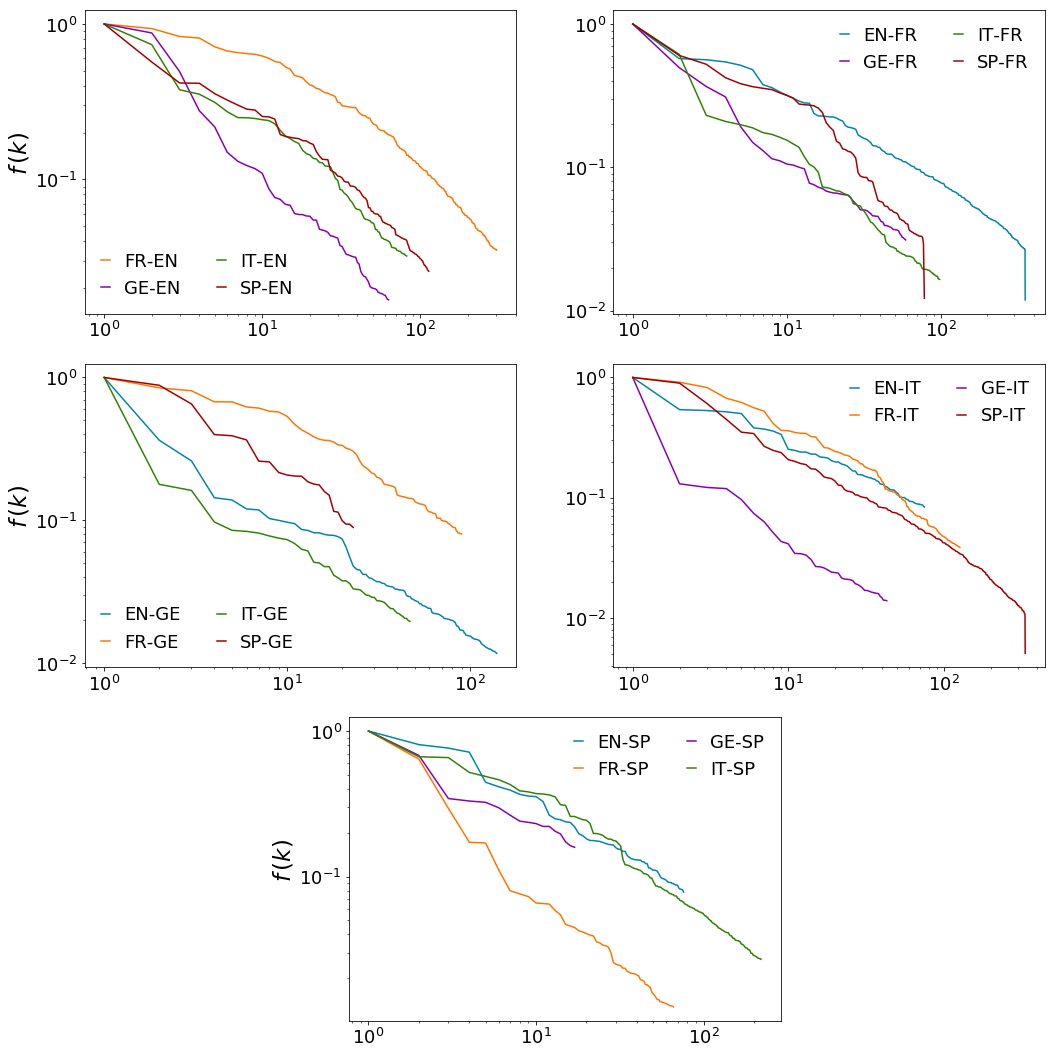
\includegraphics[scale=.38]{ZL_receptor.png}
		\caption{{\bf Zipf's law of the accumulated migrant words, grouped by receiving language.\cgnote{m\'as que Zipf's law, distribuci\'on de frecuencias, se podr\'ia hacer ajuste con Zipf e indicar exponente.}} }
		\label{fig.ZL_receiving}
	\end{adjustwidth}
\end{figure}


Another way to tell the previous deduction, is thinking that if the sum of
frequencies is the same in two sets, where the first is made up of words with
low ranks, and the second by words with high ranks, the second set would have
to have more items than the first. With these ideas, in each source language
and receiving language pair, we carry out two types of elimination, in the
first we begin to eliminate the words with the lowest ranks and little by
little increasing the portion of words eliminated $R_{p}$ (from 1$\%$ to a
99$\%$) until the words with the highest ranks are were covered
Fig~\ref{fig.RP_low}; the second way was the opposite case, beginning to
eliminate a small portion of those words with highest ranks and gradually
increasing it until cover the lower ranks Fig~\ref{fig.RP_high}. In both cases,
each time the eliminated portion was increased, the average difference was
calculated to observe the similarity.


\begin{figure}[!h]
	\begin{adjustwidth}{-2.5cm}{1cm}
		\centering
		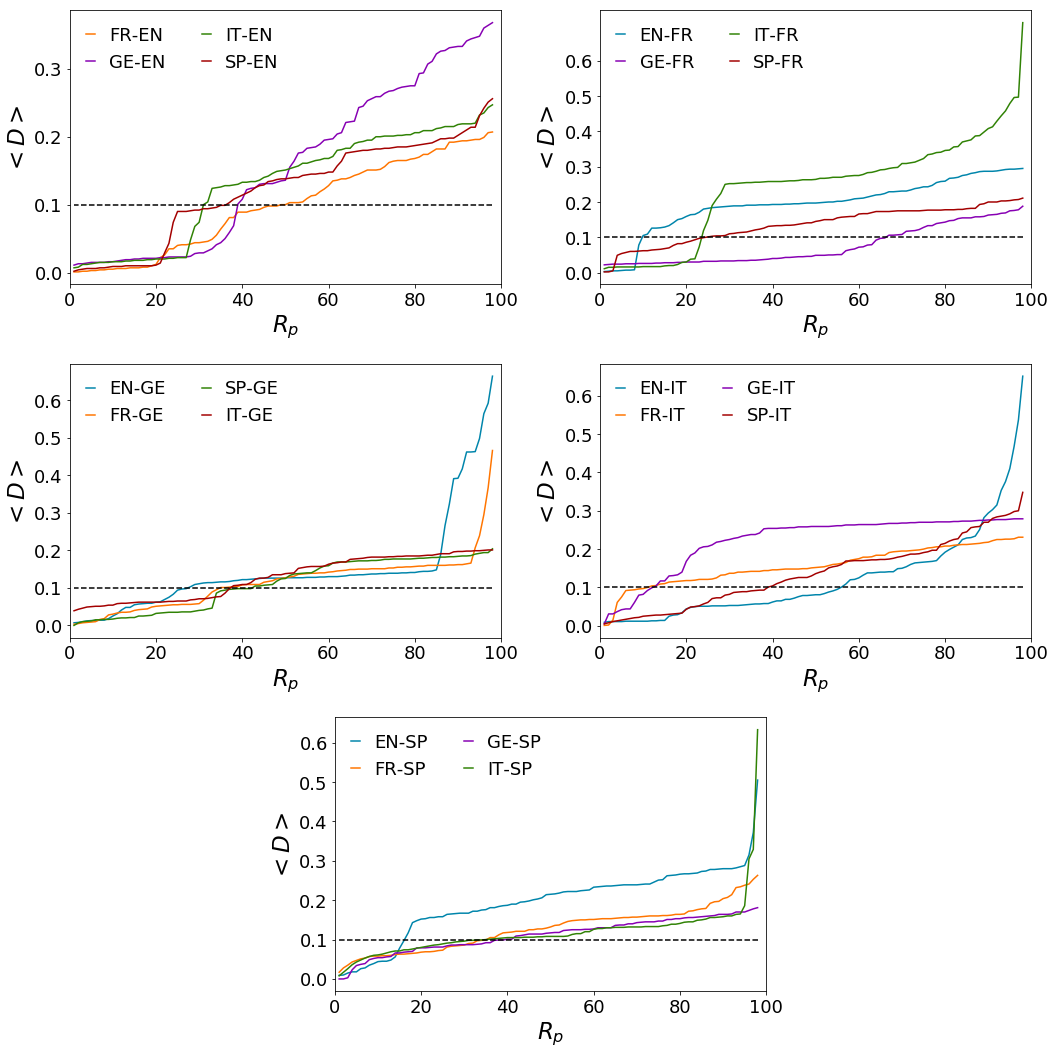
\includegraphics[scale=.38]{Rp_bajos.png}
		\caption{{\bf Portion of eliminated words with lows ranks.} }
		\label{fig.RP_low}
	\end{adjustwidth}
\end{figure}


\begin{figure}[!h]
	\begin{adjustwidth}{-2.5cm}{1cm}
		\centering
		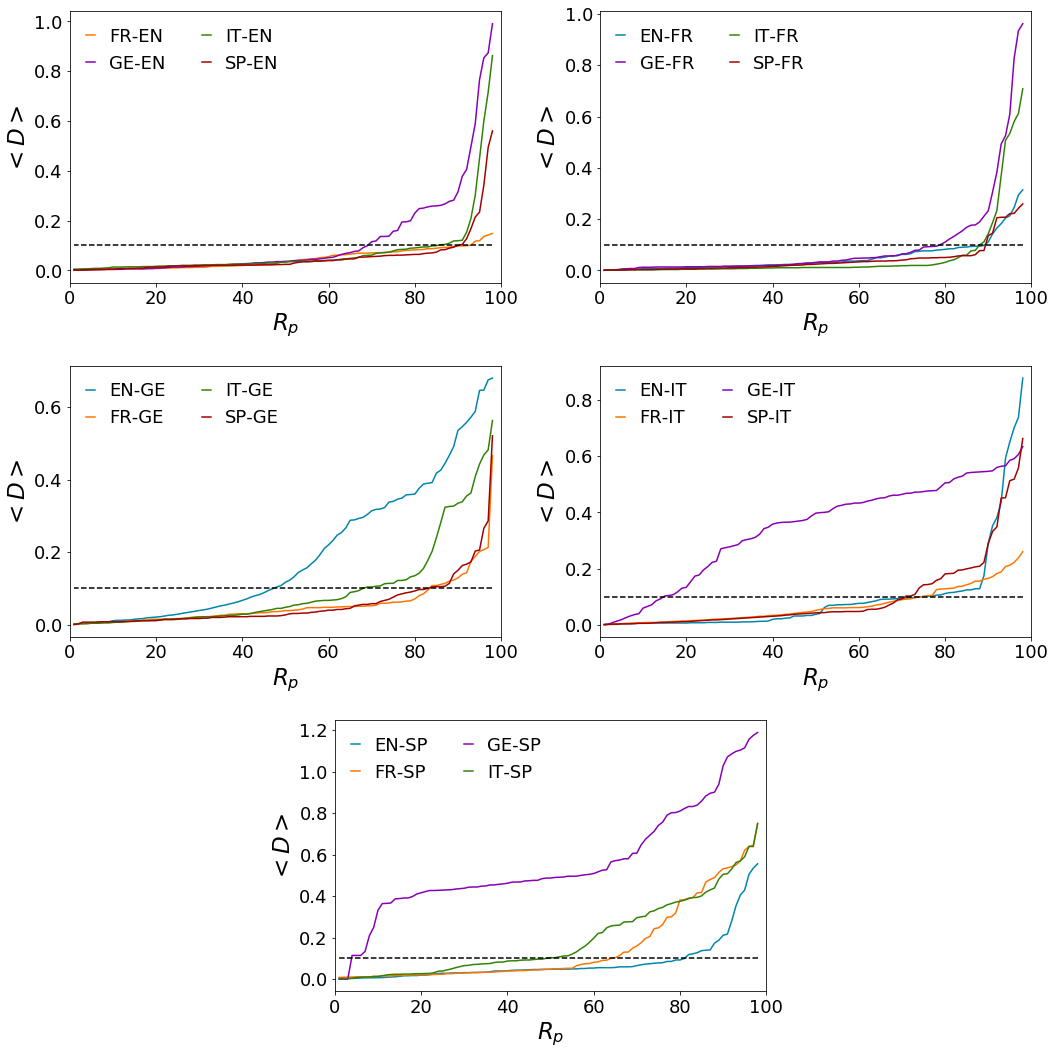
\includegraphics[scale=.38]{Rp_altos.png}
		\caption{{\bf Portion of eliminated words with high ranks.} }
		\label{fig.RP_high}
	\end{adjustwidth}
\end{figure}

After observing both figures, it is appropriate to say that for the similarity of the use between languages are altered, a greater number of words with high ranks are needed than words with low ranks, in terms of robustness, the sets are more stable if altering them are eliminated those words with the highest ranks, that is, those with the lowest frequencies.

This result, despite showing the stability of the sets when eliminating words from them, can be counterproductive with the results of the previous sections, since in those we try to find relationships based on the meaning of the words, and in case of an elimination such relationships would be lost if the words involved have high ranks.

%just multiply the original use by the conversion factor to obtain the reduced use. 

% }}}
\section*{Conclusiones} % {{{
\cpnote{Vas CarlosG}
% }}}
\section*{Supporting information} % {{{
% }}}
\section*{Acknowledgments} % {{{

\nolinenumbers

Support by projects CONACyT 285754 and UNAM-PAPIIT IG101421 is acknowledged. 
% }}}
% \bibliographystyle{plos2015}
\bibliography{referencias} 
\end{document}
